% To add an image or include a .tex file you need to add
% \CWD
% to the relative (to the main document) path.
%
% Example:
% \begin{figure}
%   \centering
%   \includegraphics{\CWD/images/example.pdf}
% \end{figure}
“O andar do bêbado” é um problema muito conhecido na matemática. Nesse problema temos um bêbado iniciando na origem do plano 2D e, a cada momento, ele escolhe aleatóriamente uma direção para andar: norte (N), sul (S), leste (L) ou oeste (O). Apesar do andar caótico, é matemáticamente garantido que o bêbado sempre volta pra a origem, sua casa!

Aqui temos um problema ligeiramente diferente, além de andar nas direções N, S, L e O, em um movimento o bêbado também pode andar na direção nordeste (NE), sudeste (SE), noroeste (NO) e sudoeste e (SO). 

Dado um número $K$, o número de passos do bêbado, imprima de quantas formas o bêbado pode fazer $K$ movimentos e terminar em casa módulo $1000000007$ ($10^9 + 7$).

\begin{figure}[H]
    \centering
    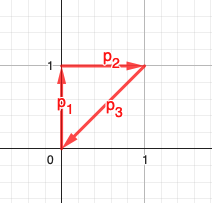
\includegraphics[width=5cm]{\CWD/andar-trebado-img.png}
    \caption{Exemplo do bêbado voltando para casa após três movimentos: N, L e SO}
\end{figure}

% For input, use one of the following
%

\inputdesc{A entrada é composta por um único inteiro $K$ ($1 \leq K \leq 5000$).}
%
% For output, use one of the following
%

\outputdescline{A saída deve ser composta por um único número: o número de formas que o bêbado pode voltar para a origem depois de $K$ movimentos módulo $10^9 + 7$.}

%\sampleio will look for files named sample-n.in and sample-n.sol (where n is 1, 2, 3...)
%in the documents directory and include them as samples.

\sampleio
